\begin{frame}
	\frametitle{Diagonalisierung als Beweistechnik}
	\framesubtitle{Diagonalisierung : Was ist das eigentlich?}
	
	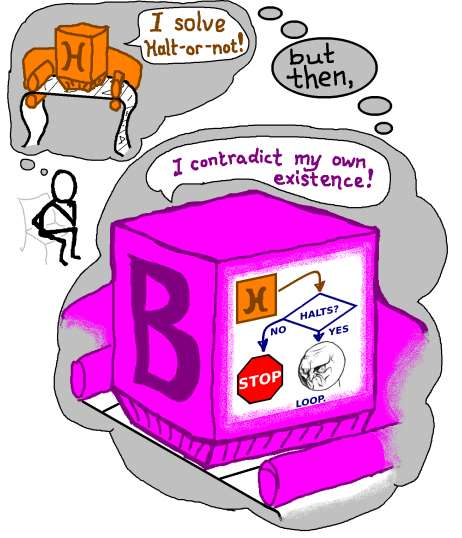
\includegraphics[scale = 0.3]{halting-problem.jpg}
\end{frame}
\begin{frame}
	\frametitle{Diagonalisierung als Beweistechnik}
	\framesubtitle{Eine Hierarchie von Komplexitätsklassen}
	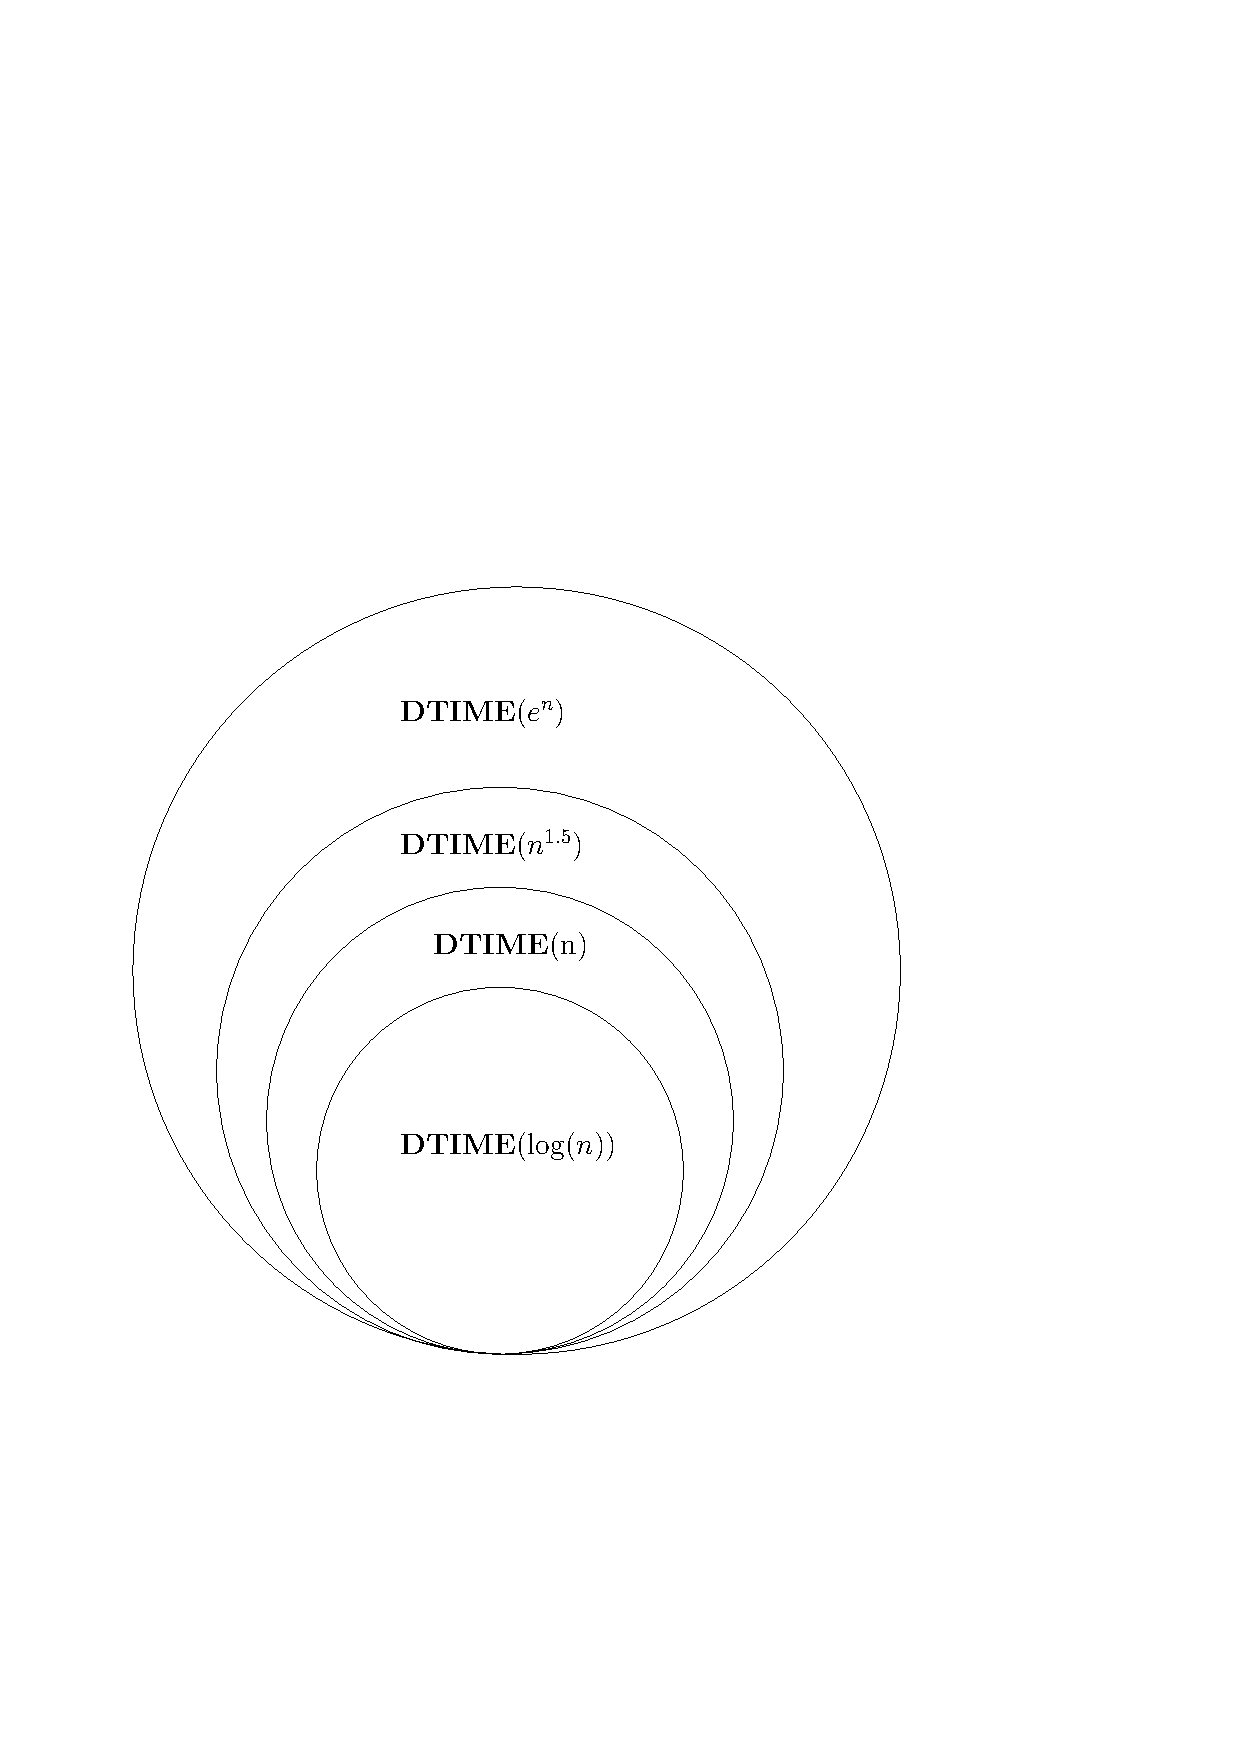
\includegraphics[scale=0.5]{images/timehierarchy.pdf}
\end{frame}
\begin{frame}
	%\frametitle{Einleitung}
	\framesubtitle{$\P$ oder $\NPC$ : gibt es noch mehr in $\NP$?}
	\overprint{
		\only<1>{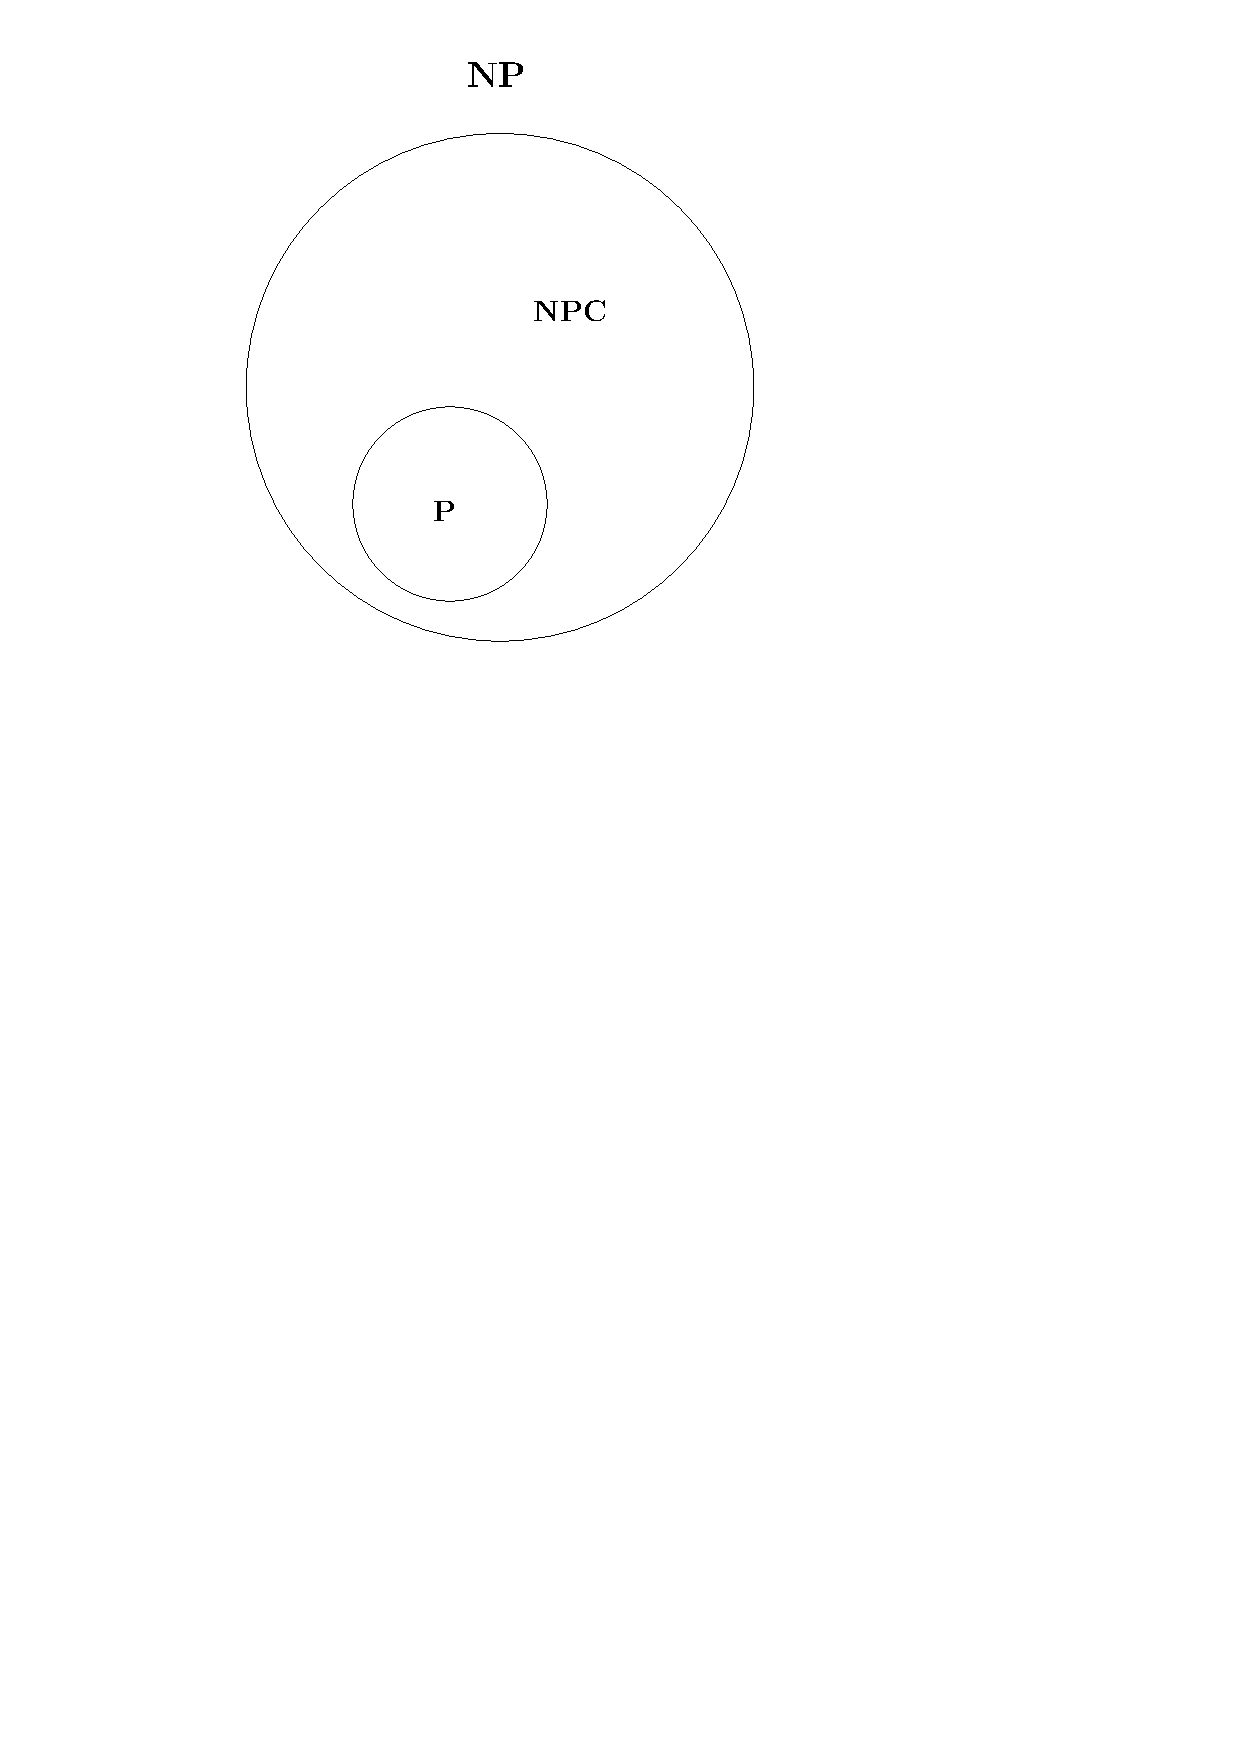
\includegraphics[page = 1,scale = 0.6]{images/npi.pdf}}
		\only<2>{\includegraphics[page = 2,scale = 0.6]{images/npi.pdf}}
	}
\end{frame}
\begin{frame}
	\frametitle{Diagonalisierung als Beweistechnik}
	\framesubtitle{Grenzen der Diagonalisierung}
	
	\begin{itemize}[<+->]
	  \item Orakelmaschinen und die P, NP Frage
	\end{itemize}
\end{frame}
\begin{frame}
	\frametitle{Die polynomoielle Hierarchie}
		\begin{itemize}[<+->]
			\item Verallgemeinerung von $\P-\NP$
			\item Kollabiert die $\PH$?
		\end{itemize}
	\end{frame}
	
	